\section{Introduction}

Grammar inference, also known as grammar induction, consists of inferring a grammar from a set of examples~\cite{horning1969study,de2010grammatical,Stevenson_Cordy_2014,D_Ulizia_Ferri_Grifoni_2011}. It has been studied and used in various fields, such as natural language processing, where it can reduce the effort required to generate syntactic or semantic models automatically~\cite{kai2024leveraginggrammarinductionlanguage, Dulizia2011A}, and software engineering, where inferred grammars can guide reverse engineering and automated parser generation~\cite{Stevenson2014A}. By relying on characteristic examples~\cite{de2010grammatical}, grammar inference enables automated discovery of underlying syntactic or structural patterns. 

\begin{figure}[t]
  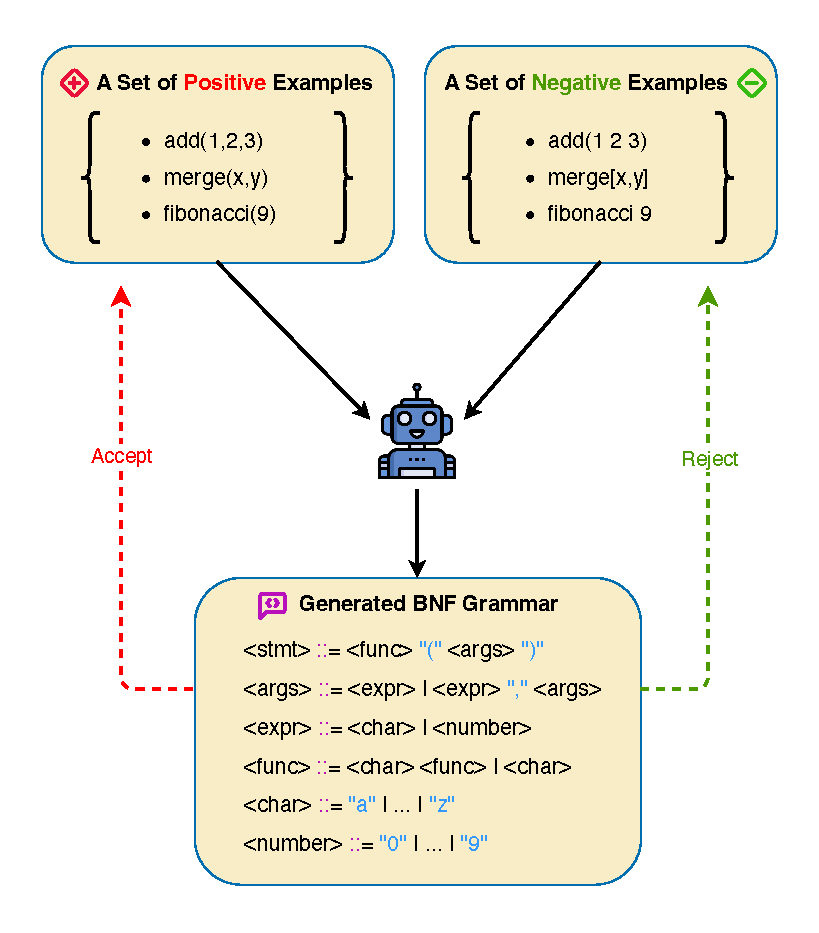
\includegraphics[width=\columnwidth]{figures/bnf_generation.pdf}
  \caption{Given a small set of positive and negative examples, LLMs should infer and generate a grammar that accepts all positives and rejects all negatives.}
  \label{fig:bnf_generation}
\end{figure}

Backus-Naur Form (BNF) is used to define the grammar of formal languages~\cite{Chomsky_1956,backus1959syntax,backus1960report}, typically Context-Free Grammars (CGFs)~\cite{Chomsky_1956, Aho_Aho_2007}. It has also been used in various ways such as in parser generators like ANTLR4~\cite{ANTLR4} and Yacc~\cite{Johnson1978YaccYA} or in constraining output structure of Large Language Models (LLMs)~\cite{willard2023efficientguidedgenerationlarge,BeurerKellner2024GuidingLT}.

Although LLMs have exhibited remarkable capabilities across diverse domains~\cite{gaur-saunshi-2023-reasoning,imani-etal-2023-mathprompter,Pan_Albalak_Wang_Wang_2023,tang2024tom,LLM-SYGUS,jiang2024surveylargelanguagemodels}, their capacity for grammar inference, and particularly for generating grammars in BNF, has not yet been well explored. This paper focuses on investigating and improving the ability of LLMs to infer a CFG and generate it in BNF from a given set of positive and negative examples. A correctly generated grammar should accept all positives and reject all negatives. Typically, grammar inference requires a large set of characteristic examples that can uniquely identify a CFG~\cite{de2010grammatical}. However, we instead explore whether LLMs can infer a CFG from fewer examples without imposing any constraints on the examples, based on their experience and knowledge acquired through training on large-scale corpora. We refer to this process as ``few-shot grammar generation'', emphasizing both the grammar inference of CFGs with fewer examples and their generation in BNF, and we use ``grammar'' to denote a CFG represented in BNF. An example is shown in Figure~\ref{fig:bnf_generation}.

To explore the capacity of LLMs for few-shot grammar generation, we first construct a dedicated dataset of 540 challenges, each with only 3 positive and 3 negative examples, and use it to evaluate the performance of 8 LLMs, encompassing both open- and closed-source models of varying parameter sizes, including those specialized for code generation. We then propose an LLM-driven hybrid genetic algorithm, namely \NAME, which adapts the principles of genetic algorithms with the integration of LLM-driven population initialization and mutation. We devised and adopted 6 metrics to comprehensively evaluate and analyze their performance from the perspectives of syntax and semantic correctness, over-fitting, over-generalization, and utility. The results show that, while most LLMs demonstrate unsatisfactory performance, our proposed algorithm significantly enhances the grammar generation ability across most of the evaluated LLMs.

We summarize the main contributions of this paper as follows:
\begin{enumerate}
    \item We constructed a dedicated dataset of 540 challenges for few-shot grammar generation and comprehensively evaluated 8 LLMs;
    \item We designed 6 metrics for measuring the ability of LLMs in this task and performed an extensive analysis based on them; 
    \item We proposed a novel method, \NAME, to improve the grammar generation performance of LLMs and showed that it achieves significant improvements across LLMs.
\end{enumerate}
